\section{Results Comparison and Analysis}
\label{cha:results}

In this chapter we evaluate the four previously defined direct 0--1
loss optimization algorithms (BnB, PCS, CSA, and SLA) on a variety of
real and synthetic data.  We compare to SVMs and logistic regression
using LibLinear~\cite{linearSVM}\footnote{Available at:
  \url{http://www.csie.ntu.edu.tw/~cjlin/liblinear}}.  We also compare
to the Bayes point machine~\cite{bpm}\footnote{Available at:
  \url{http://research.microsoft.com/en-us/um/people/minka/papers/ep/bpm}}
which is an approximate Bayesian approach with connections to the 0--1
loss.

All tests in this thesis are implemented in MATLAB 7.12.0 running on a
1.7GHz dual-core i5 Intel processor and 4GB RAM.

Synthetic testing datasets are generated as follows: 
\begin{enumerate}
  \setlength{\itemsep}{4pt}
  \setlength{\parskip}{1pt}
  \setlength{\parsep}{1pt}
	\item A common data range $R$ is randomly select between 5 and 10. 
	\item Two center points $C_1, C_2$, each corresponding to one class, are randomly chosen in the range $\pm (R/2)$ from the origin. 
	\item Variances in every dimension of the two center points $C_1, C_2$ are specified randomly in range $[1, R^2]$. 
	\item The desired number of data points for each class are then generated by a normal distribution with mean at $C_1$ or $C_2$ respectively, and a covariance matrix having corresponding variances on the main diagonal and 0 elsewhere.     
	\item If a specific range of 0--1 loss value is required. The dataset is repeatedly generated by the above step, and then checked by PCS algorithm until its 0--1 loss value is within the desired range.
\end{enumerate}

Some tests use real-world datasets, which are taken from the UCI
machine learning repository by \cite{ucidata}. These datasets are
listed in Table \ref{tab:datasets}.

%%%%%%%%%%%%%%%%%%%%%%%%%%%%%%%%%%%%%%%%%%%%%%%%%%%%%%%%%%%
\begin{table*}[htbp!]
\centering
{\footnotesize
\begin{tabular}{c  c c l}
\hline\hline
Dataset & $N$ & $D$ & Name \& Source \\
\hline
Breast & 683 & 10 & Breast Cancer, \cite{breast} \\
Liver & 345 & 6 & Liver Disorders, UCI \\
Cmc & 1473 & 9 & Contraceptive Method Choice, UCI\\
Heart & 270 & 13 & Statlog (Heart), UCI\\
Indian & 583 & 10 & Indian Liver Patient, UCI\\
Pima & 768 & 8 & Pima Indians Diabetes, UCI\\
Sonar & 208 & 60 & Connectionist Bench (Sonar, Mines vs. Rocks), UCI\\
\hline\hline
\end{tabular}}
\caption{Size, name, and source of real-world testing datasets.} 
\label{tab:datasets}
\end{table*}
%%%%%%%%%%%%%%%%%%%%%%%%%%%%%%%%%%%%%%%%%%%%%%%%%%%%%%%%%%%

The following are common procedures for data preprocessing and noise
generation.  \emph{Data preprocessing:} if not otherwise stated, all
testing datasets use standardized features (data are normalized
features-wisely to have mean-0 variance-1 before being passed as an
input to any algorithm).  emph{Noise:} If it is mentioned that a
certain percentage of noise is added to the dataset, then this step is
done prior to data preprocessing. Noise is generated randomly and
uniformly in the range from $min - 0.5(max-min)$ to $max +
0.5(max-min)$ of each dimension of the dataset, where $min, max$ are
minimum and maximum value of data in the given dimension. Noise is
then assigned to the first class of the dataset. Because the range of
noise is twice the range of data, this process produces both
background noise and outliers.

\subsection{Comparison with Other State-of-the-Art Methods}
\label{sec:rc.others}

Arguably, the most commonly used methods for binary linear
classification are logistic regression (LR) and support vector
machines (SVM). Beside those, Bayes point machines (BPM) is another
state-of-the-art method, which is gaining popularity in binary
classification. In this section, the novel algorithms shall be
compared with these existing algorithms in different tests using both
synthetic and real world datasets. The first two subsections here
contain tests aiming at pointing out the differences in optimality of
the returned solutions. It was mentioned at the beginning of the
thesis that classification based on 0--1 loss is robust to
outliers. Thus, the third subsection is devoted to comparing the
prediction accuracy of the novel algorithms with existing algorithms
in the presence of outliers. The last subsection examines a class of
datasets termed anti-surrogate-loss, for which all algorithms based on
surrogates to 0--1 loss give poor results, whereas novel algorithms
work well.


%=========================

%%%%%%%%%%%%%%%%%%%%%%%%%%%%%%%%%%%%%%%%%%%%%%%%%%%%%%%%%%%%%%%
\begin{figure*}[ht!]
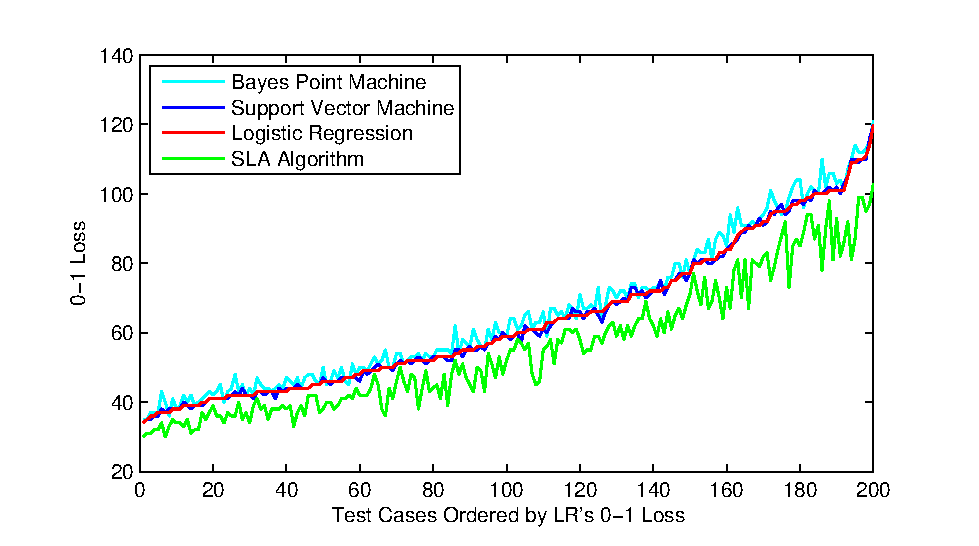
\includegraphics[width=0.50\textwidth]{images/fig61_621a.eps}
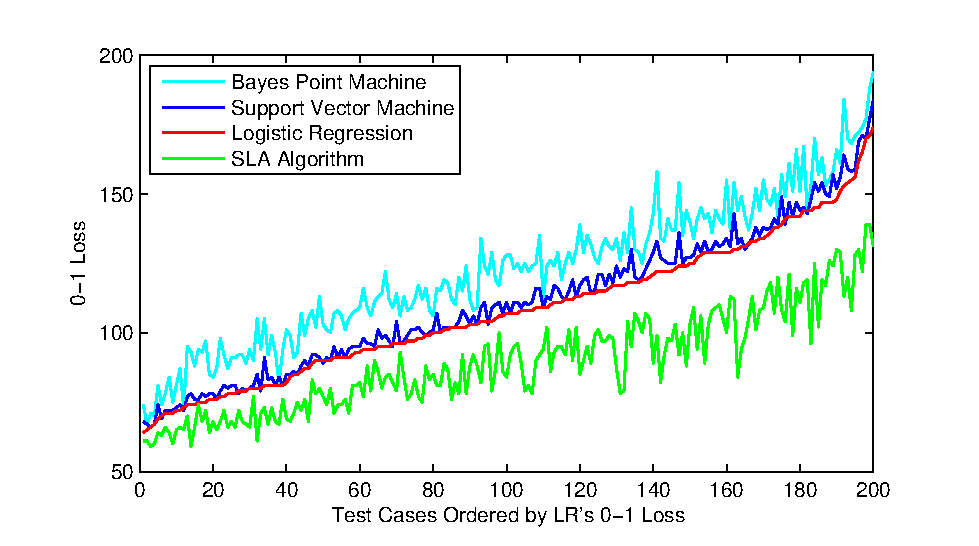
\includegraphics[width=0.50\textwidth]{images/fig61_621b.eps}
\caption{ (left) This plot shows the 0--1 loss values by SLA algorithm
  comparing to other methods over 200 synthetic datasets of $N=500,
  D=5$ with optimal 0--1 loss in the range of $[30, 100]$.  
  (right) his plot shows the 0--1 loss values returned by the
  comparing methods in presence of 15\% noise.}
\label{fig:621a}
\end{figure*}
%%%%%%%%%%%%%%%%%%%%%%%%%%%%%%%%%%%%%%%%%%%%%%%%%%%%%%%%%%%%%%%

\noindent\emph{Optimality of Solutions on Synthetic Data: }
Firstly, to see the differences in returned 0--1 loss values of
comparing algorithms. A test has been designed as follows. 200
datasets are generated with size $N=500$, dimensionality $D=5$, and
optimal 0--1 loss in the range from 30 to 100. After preprocessing,
these datasets are tested with each of the four methods and the 0--1
loss values of the solutions returned by each method are
recorded. Figure \ref{fig:621a} (top) shows the results of this test.
Secondly, to see how well different algorithms deal with noise and
outliers, another test has been designed, in which datasets are
generated the same way as in the previous test, except that 15\% of
noise (including outliers) is added to every dataset, increasing its
size to $N=575$. Figure \ref{fig:621a} (bottom) visualizes the results of this
test. The immediate thing to note in this figure is that the SLA curve
is significantly lower than other curves, and it also increases at a
slower rate. Clearly, the presence of noise and outliers influenced
other algorithms to a much greater extend than SLA. 

%=========================

%%%%%%%%%%%%%%%%%%%%%%%%%%%%%%%%%%%%%%%%%%%%%%%%%%%%%%%%%%%%%%
\begin{table*}[htbp!]
\centering
{\footnotesize 
\begin{tabular}{|cc|  ccc|cccc|c|}
\hline\hline
{\bf Dataset} && {\bf BPM} & {\bf SVM} & {\bf LR} & {\bf SLA} & {\bf CSA} & {\bf PCS} & {\bf BnB} & {\bf \% }\\ 
\hline 
Breast	&& 19 & 18 & 19 & 13 		& 13 & 19 & 10 & 44.4\%\\  
Bupa		&& 104 & 99 & 99 & 89 		& 91 & 91 & 95 & 10.1\%\\   
Cmc		&& 468 & 464 & 468 & 418 	& 429 & 459 & 459 & 9.9\%\\   
Heart  	&& 38 & 39 & 39 & 27 		& 31 & 33 & 25 & 34.2\%\\  
Indian  	&& 153 & 154 & 154 & 146 	& 154 & 154 & 148 & 4.6\%\\    
Pima 	&& 164 & 166 & 166 & 156 	& 157 & 159 & 161 & 4.9\%\\    
Sonar  	&& 16 & 0 & 0 & 0 			& 0 & 0 & 0 & 0\%\\ 
\hline\hline
\end{tabular}}
\caption{0--1 loss values of comparing algorithms on original
  data. Column `{\bf \%}' shows the improvement in percentage of the
  best of novel algorithms (SLA, CSA, PCS, BnB) over the best of
  existing algorithms (BPM, SVM, LR). As can be seen, novel algorithms
  represent a significant improvement in 0--1 loss optimization.}
\label{tab:losses0noise}
\end{table*}
%%%%%%%%%%%%%%%%%%%%%%%%%%%%%%%%%%%%%%%%%%%%%%%%%%%%%%%%%%%%%%%%


%%%%%%%%%%%%%%%%%%%%%%%%%%%%%%%%%%%%%%%%%%%%%%%%%%%%%%%%%%%%%%%%
\begin{table*}[htbp!]
\centering
{\footnotesize 
\begin{tabular}{|cc|  ccc|cc c| cc|}
\hline\hline
\multirow{2}*{{\bf Dataset}}&&\multicolumn{5}{c}{{\bf T1 -- Total Running Time}}&&\multicolumn{2}{c|}{{\bf T0--ReachSol.}}  \\ 
\cline{3-10}
 && {\bf BPM} & {\bf SVM} & {\bf LR} & {\bf SLA} & {\bf CSA} && {\bf PCS} & {\bf BnB}\\  
\hline
Breast && 0.98 & 0.03 & 0.05 & 1.13 & 161.64 && n/a & 3.59 \\  
Bupa && 0.28 & 0.01 & 0.01 & 0.39 & 16.11 && 97.07 & 0.17 \\  
Cmc && 1.35 & 0.06 & 0.05 & 1.02 & 312.78 && 252.06 & 153.4 \\  
Heart && 0.40 & 0.02 & 0.03 & 0.77 & 126.52 && 1.24 & 63.56 \\  
Indian && 0.76 & 0.05 & 0.04 & 1.24 & 166.10 && n/a & 0.8 \\  
Pima && 0.65 & 0.03 & 0.04 & 0.89 & 157.38 && 63.30 & 89.89 \\  
Sonar && 0.37 & 0.54 & 0.13 & 4.32 & 302.58 && n/a & n/a \\
\hline\hline
\end{tabular}}
\caption{This table reports running times corresponding to test result
  given in Table \ref{tab:losses0noise}. T1 is the total running time
  for BPM, SVM, LR, SLA, CSA (these are fast, so not time limited). T0
  is the time to reach the given solutions for PCS, BnB (their running
  time is unknown as they are terminated after 300 seconds). $T0=n/a$
  means the corresponding algorithm could not find any better solution
  than the initial approximation within the given time limit. Note
  that SVM and LR has linear running time. It can be seen, that among
  novel algorithms, SLA is significantly better than others. }
\label{tab:runningtimes}
\end{table*}
%%%%%%%%%%%%%%%%%%%%%%%%%%%%%%%%%%%%%%%%%%%%%%%%%%%%%%%%%%%%%%%%

\noindent\emph{Optimality of Solutions on Real-World Datasets:}
So that tests are not limited to synthetic data, the last test of this
section is performed on several real-world datasets taken from the UCI
machine learning repository (given in Table \ref{tab:datasets}). This
test compares the optimality of the returned solutions of all
algorithms: BnB, PCS, CSA, SLA, BPM, SVM, LR. In this test, datasets
are tested with each of the algorithms in two scenarios: without noise
and with 10\% noise. Clearly, the size of the testing datasets do not
allow an exhaustive search, hence a time threshold of 300 seconds is
set for BnB, PCS. In the case of CSA, the first layer of approximation
is set to have $N'=D+8$ and time limit $=100$ seconds. The results of
this test are shown in multiple tables as follows:
\begin{itemize}
\setlength{\itemsep}{4pt} 
\setlength{\parskip}{1pt}
\setlength{\parsep}{1pt}
\item Table \ref{tab:losses0noise} shows the 0--1 loss values returned by comparing algorithms for the original data.
\item Table \ref{tab:losses1noise} shows the results in the scenario where 10\% noise is added.
\item Table \ref{tab:runningtimes} shows the running time (T1) of BPM, SVM, LR, SLA, CSA and the time to reach the given solution (T0) of BnB and PCS.
\end{itemize}

It can be seen from the results, that novel algorithms represent a
significant improvement over existing algorithms, and the difference
is deepened in presence of noise.

Among all novel algorithms, the 0--1 loss values by SLA is comparable
or better than others, while its running time is by many times
faster. In the ``without noise'' scenario, SLA represents an average
improvement rate of 12\% over the best result of BPM, SVM, LR. In the
presence of 10\% noise, this rate is increased to 17.4\%, and can be
well over 30\% in some cases. Note that we have used a fixed setting
for parameters of SLA for all datasets, if its parameters were tuned
for each dataset, the result of SLA would have been even better. Thus,
in the next subsections, SLA is used to represent all proposed direct
0--1 loss optimization algorithms.

This subsection concentrates
on testing the accuracy of predictions given by a 0--1 loss classifier
based on SLA algorithm comparing to that given by other methods in the
presence of noise and outliers. The testing procedure is as
follows. First, 10\% noise is added to a dataset. Then, the
regularization constant of each classifier is determined by performing
5-fold cross-validation on this dataset. Note, that other parameters
for SLA algorithm are fixed at the values given by the example in
Section \ref{sec:sla.algorithm} for all datasets. Next, the dataset is
randomly split 500 times into a training set (80\% of samples) and a
test set (20\% of samples), which is then tested with each of
classifiers. The mean and standard deviation of the 200 prediction
error rates is recorded in each case to represent the average
prediction error rate of each classifier for the given dataset.

The first test is performed on 100 synthetic datasets with a wider
range of size $N \in [400, 800]$, dimensionality $D \in [4, 8]$, and
0--1 loss values from 50 to 250 (but always less than $0.3 N$ in any
specific case to avoid abnormalities). Table \ref{tab:errorrates}
shows the average statistics of these 100 test cases, where it can be
seen, that SLA give the lowest prediction error rate representing
6.75\% improvement over the best result of other methods (given by
LR), and 12.57\% over the worst (BPM).

%%%%%%%%%%%%%%%%%%%%%%%%%%%%%%%%%%%%%%%%%%%%%%%%%%%%%%%%%%%%%%%%
\begin{table*}[htbp!]
\centering
{\footnotesize 
\begin{tabular}{|cc|  ccc|c|c|}
\hline\hline
{\bf Dataset} && {\bf BPM} & {\bf SVM} & {\bf LR} & {\bf SLA} & {\bf Improvement \%.}\\  
\hline
Breast && $8.95 \pm 2.19$ & $8.42 \pm 2.30$ & $8.09 \pm 2.01$ & $6.87 \pm 1.78$ & +15.1\%\\  
Liver && $43.01 \pm 4.81$ & $42.62 \pm 4.93$ & $45.31 \pm 5.00$ & $40.86 \pm 5.71$ & +4.1\%\\  
Cmc && $35.61 \pm 2.41$ & $35.50 \pm 2.36$ & $36.14 \pm 2.37$ & $36.83 \pm 2.47$ & -3.7\%\\  
Heart && $21.14 \pm 4.72$ & $19.35 \pm 4.45$ & $19.42 \pm 4.52$ & $20.14 \pm 4.31$ & -4.1\%\\  
Indian && $26.63 \pm 3.52$ & $26.67 \pm 3.80$ & $27.13 \pm 3.43$ & $26.36 \pm 3.24$ & +2.7\%\\  
Pima && $28.38 \pm 2.99$ & $28.61 \pm 3.11$ & $28.76 \pm 2.97$ & $25.65 \pm 3.17$ & +9.6\%\\  
Sonar && $28.24 \pm 6.60$ & $28.29 \pm 5.90$ & $28.07 \pm 6.26$ & $27.71 \pm 5.67$ & +1.2\%\\[1ex]   
\hline\hline
\end{tabular}}
\caption{Prediction error rates (given in \%) of each classifier for
  each UCI dataset (with 10\% noise). The improvement column shows the
  percent improvement of SLA over the best result of other methods ($-$
  indicates SLA was worse). It can be seen that SLA offers lower held-out
  test error rates in five of the seven datasets.}
\label{tab:ucierrorrates}
\end{table*}
%%%%%%%%%%%%%%%%%%%%%%%%%%%%%%%%%%%%%%%%%%%%%%%%%%%%%%%%%%%%%%%%

The second test is performed on UCI datasets listed in Table
\ref{tab:datasets}. The error rates (in \%) for each case is listed in
Table \ref{tab:ucierrorrates} with $\pm$ one standard deviation. Note
that the 'Diff.' column shows the difference between SLA and the
minimum error rate of others (BPM, SVM, and LR). For instance, in the
case of Pima dataset, SLA error rate is 25.65\%, by $2.73$ lower than
the minimum $28.38$ of others. As can be seen, SLA has lower
prediction error rates than others in all cases, except for the Cmc
and Heart dataset. For completeness, the corresponding prediction
error rates for the original data (without added noise) are given in
Table \ref{tab:ucierrorrates2}, where we see that SLA consistently
gives better results than any other algorithm individually. 
